\section{Results}\label{sec:results}

\subsection{Study Population, Record Audit, Excluded Categories and Common Support}\label{sec:res-cohort}

Among 66,713 NORS outbreak records, 11,358 were foodborne outbreaks in 2009--2023, of which 4,133 outbreaks (103,040 cases) had confirmed etiology in one of six study groups: \textit{Salmonella} (1,758 outbreaks; 47,779 cases), norovirus GII (1,206; 29,712), STEC (388; 5,818), norovirus GI (297; 7,998), \textit{Campylobacter} (296; 3,254) and \textit{C. perfringens} (188; 8,479) (Figure~\ref{fig:flow}). Overall, 3,908 eligible outbreaks had a single etiology entry and 225 had multiple entries within one group. Auditing found zero arithmetic contradictions; 3,976 outbreaks (95,781 cases) were complete-field consistent and 157 (7,259 cases) had blank outcome fields (52 blank $K_i$, 28 blank $H_i$ with $K_i=0$, 23 blank $H_i$ with $K_i>0$, and 54 both blank; Supplementary Table S1), leaving 19.4\% of eligible cases with unrecorded status.

Three excluded foodborne groups were profiled separately (Supplementary Table S2): 951 suspected study-group outbreaks (12,965 cases; median 6 [IQR 3--14]; recorded hospitalization 1.8\%; unrecorded status 13.5%), 304 confirmed norovirus outbreaks lacking genogroup specification (7,679 cases; median 16 [8--28]; 1.0\% hospitalized; 20.6\% unrecorded), and 300 mixed or non-study multi-agent outbreaks (8,480 cases; 4.0\% hospitalized; 15.8\% unrecorded; including 104 with $\ge 1$ confirmed study group, 4,541 cases). Twelve of 21 setting--period cells met the common-support threshold ($\ge 3$ outbreaks per group), retaining 3,176 outbreaks (76.8\%) and 72,132 cases (70.0\%; 61.0\% for \textit{Salmonella} and 67.8\% for STEC to 77.5\%--81.3\% for the other four groups; Supplementary Table S3; Supplementary Figure S1).

\begin{figure}[!tbp]
  \centering
  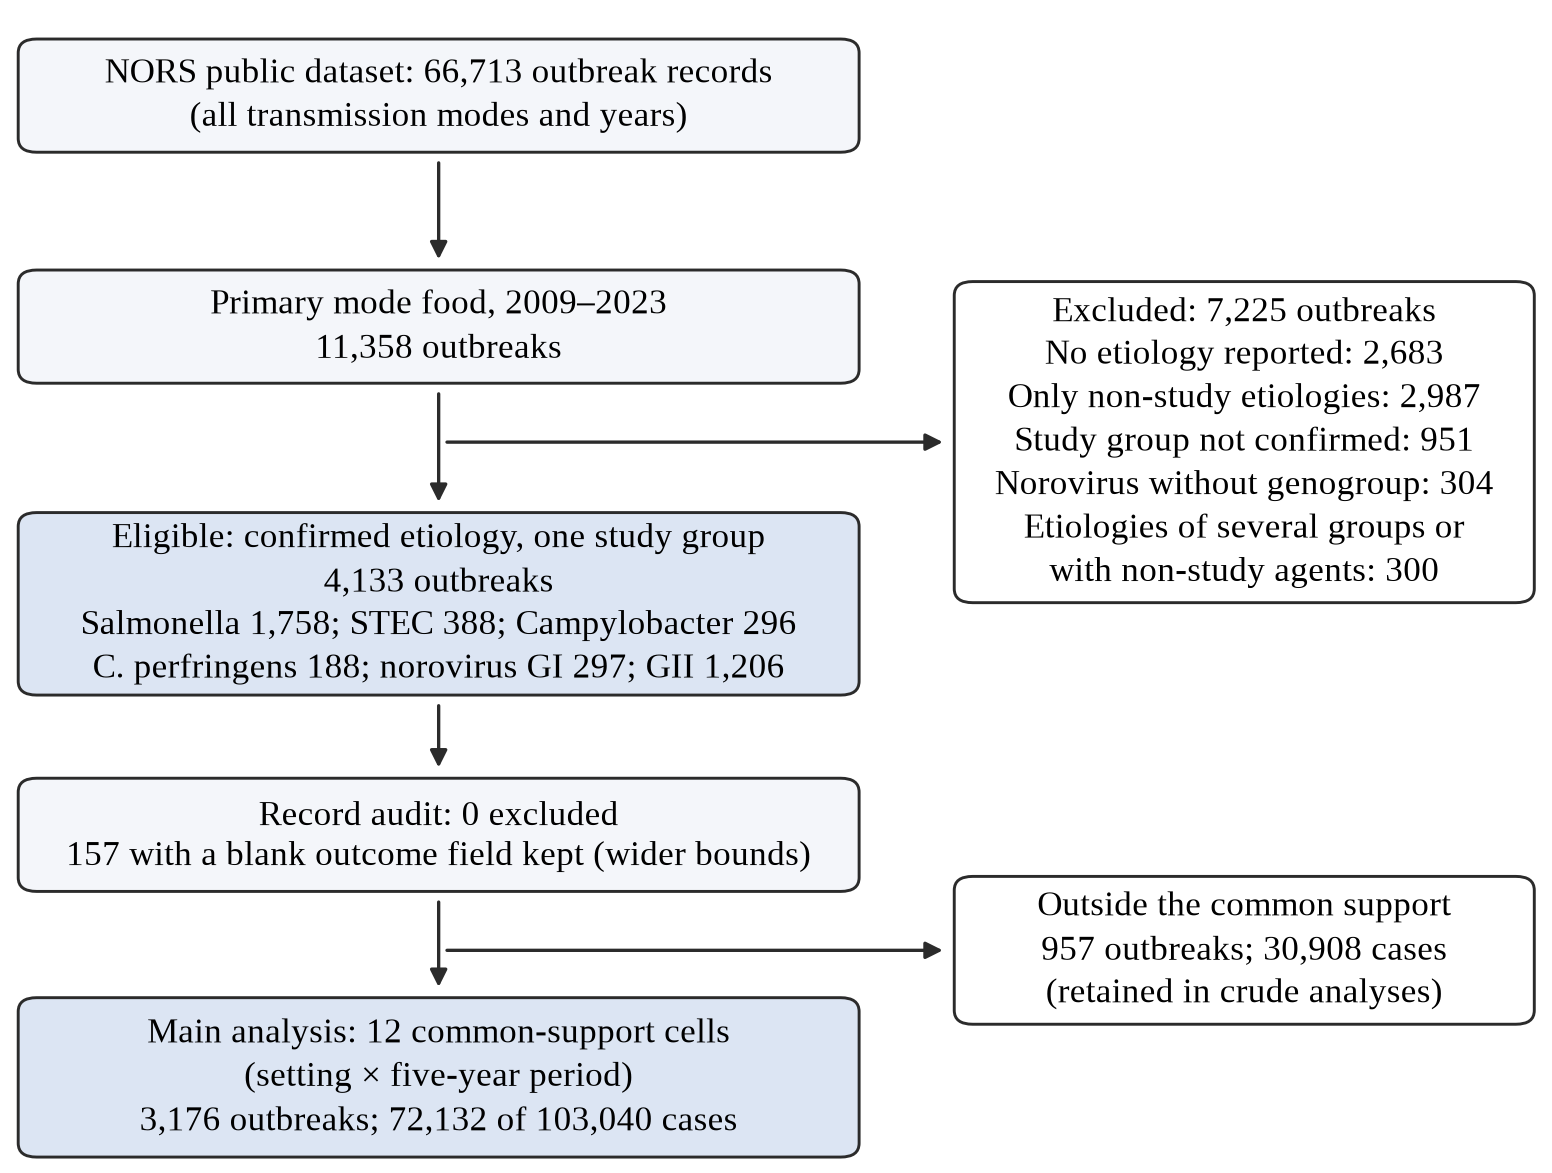
\includegraphics[width=0.82\linewidth]{figures/fig_01_selection_flow.png}
  \caption{Selection of confirmed foodborne outbreaks across six pathogen groups in NORS, United States, 2009--2023. All 157 eligible outbreaks with blank hospitalization fields were retained under logical bounds.}
  \label{fig:flow}
\end{figure}

\subsection{Sample Bounds, Composition-Adjusted Diagnostics and Sensitivity Stress Tests}\label{sec:res-bounds}

Under the 12-cell reference distribution, sample worst-case intervals were 24.7\%--36.8\% for STEC, 14.5\%--31.7\% for \textit{Salmonella}, 7.4\%--19.3\% for \textit{Campylobacter}, 1.3\%--17.2\% for norovirus GII, 0.4\%--19.7\% for \textit{C. perfringens} and 0.4\%--18.7\% for norovirus GI (Table~\ref{tab:group_bounds}; Figure~\ref{fig:intervals}, showing crude $H/C$ and $H/K$ values overlaid). Standardized $\delta = 0$ values lay at 28.5\%, 17.6\%, 8.5\%, 1.6\%, 0.6\% and 0.5\%, respectively. Without assumptions on unrecorded hospitalization outcomes, 4 of 15 pairwise orderings were determined in the sample: STEC exceeded \textit{Campylobacter} (by 5.5 percentage points), \textit{C. perfringens} (5.0 points), norovirus GI (6.0 points) and norovirus GII (7.5 points) (Figure~\ref{fig:verdicts}; Table~\ref{tab:pairwise}). Under illustrative symmetric departures, 14 orderings held at $\delta = 1$ and $2$ points and 12 held at $\delta = 5$ and $10$ points; eight sample-undetermined orderings---STEC above \textit{Salmonella} ($\delta^{*} = 41.3$ points), \textit{Salmonella} above the four lower groups (51.1--81.6) and \textit{Campylobacter} above the lowest three (35.5--37.8)---held across wide bands, whereas all three orderings among norovirus GII, \textit{C. perfringens} and norovirus GI failed below 5 points ($\delta^{*} = 4.2$, $3.7$ and $0.19$ points).

\begin{figure}[!tbp]
  \centering
  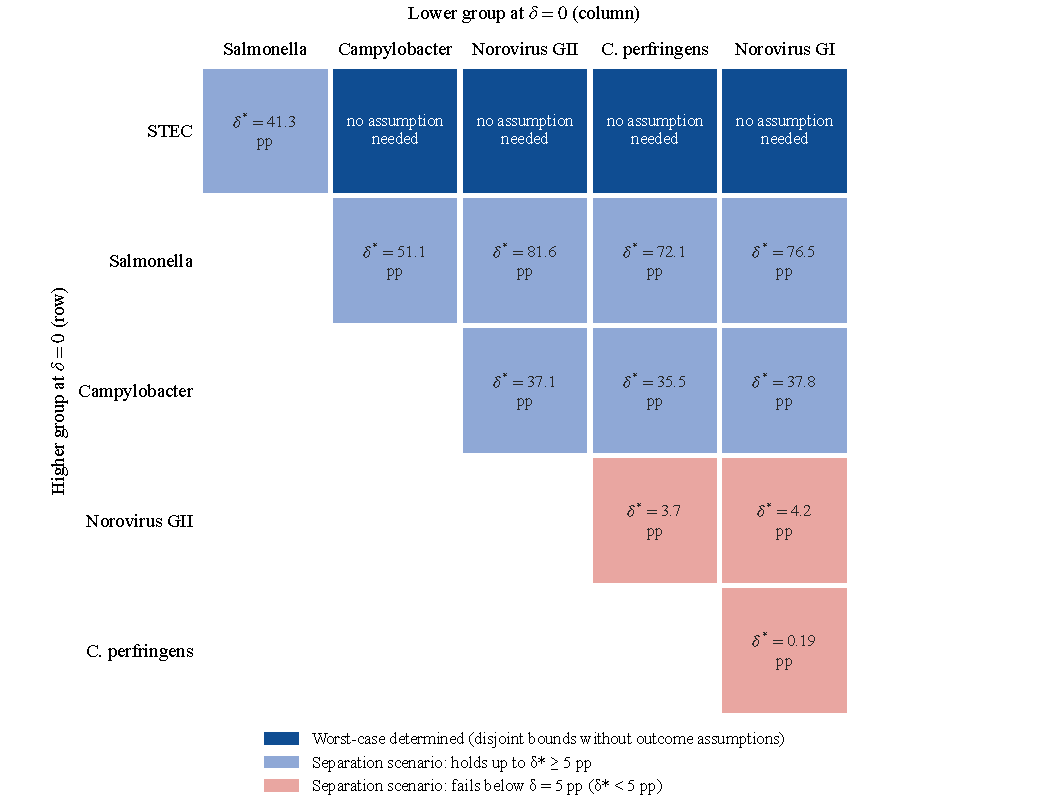
\includegraphics[width=0.80\linewidth]{figures/fig_02_verdict_matrix.pdf}
  \caption{Sample pairwise orderings and critical deviations $\delta^{*}$ across six pathogen groups, NORS foodborne outbreaks, United States, 2009--2023. Dark blue cells hold without assumptions on unrecorded outcomes; light blue and light red cells partition pairs relative to the illustrative scenario threshold $\delta = 5$ percentage points.}
  \label{fig:verdicts}
\end{figure}

\begin{table}[!tbp]
\centering
\scriptsize
\setlength{\tabcolsep}{3pt}
\renewcommand{\arraystretch}{1.12}
\caption{Standardized hospitalization proportion among reported outbreak cases, by pathogen group (12 common-support setting $\times$ period cells, pooled-case reference weights). Sample worst-case intervals are identification intervals; bootstrap ranges are the 2.5th--97.5th percentiles of each bound over 2,000 outbreak-level resamples.}
\label{tab:group_bounds}
\begin{tabular}{>{\raggedright\arraybackslash}p{2.0cm}>{\raggedleft\arraybackslash}p{1.4cm}>{\raggedleft\arraybackslash}p{1.1cm}>{\raggedleft\arraybackslash}p{1.4cm}>{\raggedleft\arraybackslash}p{1.6cm}>{\raggedleft\arraybackslash}p{1.5cm}>{\raggedleft\arraybackslash}p{1.2cm}>{\raggedleft\arraybackslash}p{1.8cm}>{\raggedleft\arraybackslash}p{1.8cm}}
\toprule
Group & Outbreaks & Cases & Unrecorded status (\%) & Worst-case interval (\%) & $\delta$ = 5 interval (\%) & $\delta$ = 0 value (\%) & Bootstrap range of lower bound (\%) & Bootstrap range of upper bound (\%) \\
\midrule
STEC & 268 & 3,943 & 12.7 & 24.7--36.8 & 27.9--29.1 & 28.5 & 21.7--29.3 & 32.6--42.3 \\
Salmonella & 1,277 & 29,151 & 18.1 & 14.5--31.7 & 16.8--18.5 & 17.6 & 13.3--15.9 & 28.2--35.5 \\
Campylobacter & 237 & 2,644 & 14.5 & 7.4--19.3 & 7.9--9.1 & 8.5 & 6.2--9.6 & 14.2--24.4 \\
Norovirus GII & 1,002 & 23,356 & 16.5 & 1.3--17.2 & 1.3--2.4 & 1.6 & 1.1--1.6 & 12.9--20.8 \\
C. perfringens & 147 & 6,568 & 22.2 & 0.4--19.7 & 0.4--1.6 & 0.6 & 0.2--0.9 & 8.5--28.1 \\
Norovirus GI & 245 & 6,470 & 16.2 & 0.4--18.7 & 0.4--1.5 & 0.5 & 0.2--0.6 & 11.7--26.8 \\
\bottomrule
\end{tabular}
\par\smallskip\parbox{0.97\linewidth}{\footnotesize Unrecorded status is the share of retained cases whose hospitalization status was not recorded, including the C $-$ H unrecorded cases from the 52 blank-K records where K was set to H. The $\delta$ = 0 value is the proportion if unrecorded-status cases had the recorded rate of their group and cell.}
\end{table}

\begin{table}[!tbp]
\centering
\scriptsize
\setlength{\tabcolsep}{2.1pt}
\renewcommand{\arraystretch}{1.12}
\caption{Pairwise orderings with worst-case verdicts, critical additive deviations $\delta^{*}$, critical odds-ratio factors $\Gamma^{*}$, illustrative symmetric and asymmetric ($-$15/+5 pp) stress-test verdicts, and bootstrap determination shares.}
\label{tab:pairwise}
\begin{tabular}{>{\raggedright\arraybackslash}p{2.4cm}>{\raggedright\arraybackslash}p{1.55cm}>{\raggedleft\arraybackslash}p{0.92cm}>{\raggedleft\arraybackslash}p{0.95cm}>{\raggedleft\arraybackslash}p{0.6cm}>{\raggedleft\arraybackslash}p{0.6cm}>{\raggedleft\arraybackslash}p{0.6cm}>{\raggedleft\arraybackslash}p{0.65cm}>{\raggedleft\arraybackslash}p{1.1cm}>{\raggedleft\arraybackslash}p{1.4cm}>{\raggedleft\arraybackslash}p{1.4cm}}
\toprule
Ordering at $\delta$ = 0 & Worst case & $\delta^{*}$ (pp) & OR $\Gamma^{*}$ & $\delta$ = 1 & $\delta$ = 2 & $\delta$ = 5 & $\delta$ = 10 & Asym ($-$15/+5) & Boot det., worst (\%) & Boot det., $\delta$ = 5 (\%) \\
\midrule
STEC $>$ CAMP & determined & $\infty$ & $\infty$ & yes & yes & yes & yes & yes & 97.0 & 100.0 \\
STEC $>$ CPERF & determined & $\infty$ & $\infty$ & yes & yes & yes & yes & yes & 91.6 & 100.0 \\
STEC $>$ NoV GI & determined & $\infty$ & $\infty$ & yes & yes & yes & yes & yes & 93.6 & 100.0 \\
STEC $>$ NoV GII & determined & $\infty$ & $\infty$ & yes & yes & yes & yes & yes & 100.0 & 100.0 \\
SAL $>$ NoV GII & undetermined & 81.6 & 342.1 & yes & yes & yes & yes & yes & 14.2 & 100.0 \\
SAL $>$ NoV GI & undetermined & 76.5 & 1420.4 & yes & yes & yes & yes & yes & 14.5 & 100.0 \\
SAL $>$ CPERF & undetermined & 72.1 & $\infty^{\dagger}$ & yes & yes & yes & yes & yes & 24.8 & 100.0 \\
SAL $>$ CAMP & undetermined & 51.1 & 17.5 & yes & yes & yes & yes & yes & 4.2 & 100.0 \\
STEC $>$ SAL & undetermined & 41.3 & 8.41 & yes & yes & yes & yes & yes & 0.6 & 100.0 \\
CAMP $>$ NoV GI & undetermined & 37.8 & 115.9 & yes & yes & yes & yes & yes & 0.1 & 98.4 \\
CAMP $>$ NoV GII & undetermined & 37.1 & 41.2 & yes & yes & yes & yes & yes & 0.0 & 100.0 \\
CAMP $>$ CPERF & undetermined & 35.5 & 120.6 & yes & yes & yes & yes & yes & 1.8 & 100.0 \\
NoV GII $>$ NoV GI & undetermined & 4.2 & 7.75 & yes & yes & no & no & no & 0.0 & 35.2 \\
NoV GII $>$ CPERF & undetermined & 3.7 & 4.99 & yes & yes & no & no & no & 0.0 & 33.1 \\
CPERF $>$ NoV GI & undetermined & 0.19 & 1.19 & no & no & no & no & no & 0.0 & 0.0 \\
\bottomrule
\end{tabular}
\par\smallskip\parbox{0.97\linewidth}{\footnotesize Boot det. columns show the percentage of 2,000 bootstrap replicates in which the ordering is determined (non-overlapping intervals) at worst case and $\delta$ = 5 pp. $^{\dagger}$OR $\Gamma^{*}$ = $\infty^{\dagger}$ for SAL $>$ CPERF reflects 9/72 cells having zero recorded hospitalizations (p\_js = 0), which pure multiplicative scaling cannot shift upward; applying a 0.1\% continuity floor yields $\Gamma^{*}$ = 955.7 (Table S4).}
\end{table}


\begin{figure}[!tbp]
  \centering
  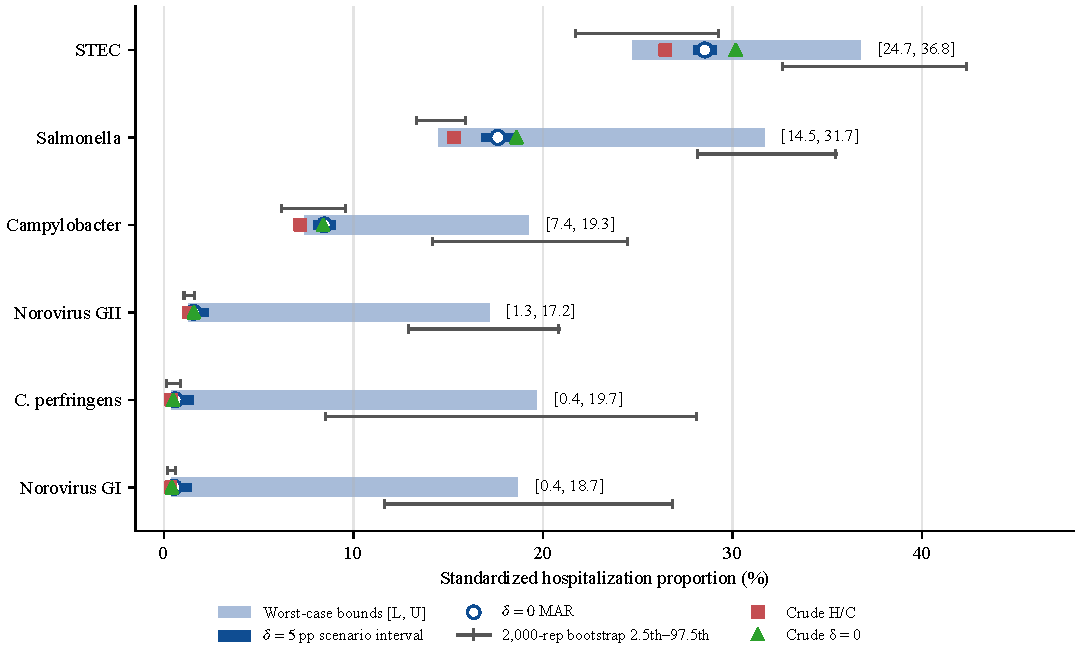
\includegraphics[width=0.92\linewidth]{figures/fig_03_bound_intervals.pdf}
  \caption{Standardized hospitalization proportions and identification intervals overlaid with crude $H/C$ (squares) and $H/K$ (triangles) conventions across the 12 common-support cells. Light bars show worst-case intervals; dark bars show the $\delta = 5$ percentage-point scenario; error bars give 2.5th--97.5th percentiles over 2,000 outbreak-level bootstrap replicates.}
  \label{fig:intervals}
\end{figure}

Comparing partially recorded ($M_i > 0, K_{\text{rec},i} > 0$) against fully recorded ($M_i = 0$) outbreaks demonstrated that large crude differences reflect outbreak composition rather than uniform outcome-dependent missingness (Supplementary Table S4). Partially recorded outbreaks were substantially larger (median 16 vs.\ 5 cases for STEC; 19 vs.\ 7 for \textit{Salmonella}) and far more often multistate (60.0\% vs.\ 11.7\% for STEC; 34.2\% vs.\ 2.4\% for \textit{Salmonella}). After cell standardization, the STEC partial-minus-full gap collapsed from $+10.93$ points to $+0.19$ points (and actually reversed within multistate outbreaks to $-1.28$ points, leaving ``Std obs $-$ Full'' $= -3.22$ points because the main $\delta=0$ anchor of 28.5\% lay below the standardized fully recorded STEC rate of 31.1\%). For \textit{Salmonella}, a $+9.02$-point within-cell difference persisted (``Std obs $-$ Full'' $= +2.86$ points) and was strongest within multistate outbreaks ($+11.98$ points vs.\ $+4.34$ single-state), coinciding with active subtype-linked surveillance rather than solely outcome-selective field recording. In 11 low-missingness states ($<5\%$ unrecorded status), recorded rates were 26.2\% (STEC), 13.0\% (\textit{Salmonella}), 8.8\% (\textit{Campylobacter}), 1.3\% (norovirus GII), 0.0\% (\textit{C. perfringens}) and 0.3\% (norovirus GI). Scenario stress tests confirmed that all 12 upper-tier orderings remain separated under asymmetric bands of $-10/+5$, $-15/+5$ and $-20/+5$ points (Figure~\ref{fig:cal2d}; Table~\ref{tab:pairwise}). Under odds-ratio scaling, 14 of 15 pairs held at $\Gamma \le 3.0$ and 13 at $\Gamma = 5.0$ both under pure multiplicative scaling and after imposing a 0.1\% continuity floor on all 9 zero-rate cells ($\Gamma^{*} = 8.41$ for STEC above \textit{Salmonella}; $\Gamma^{*} = 955.7$ vs.\ $\infty^{\dagger}$ for \textit{Salmonella} above \textit{C. perfringens}).

\begin{figure}[!tbp]
  \centering
  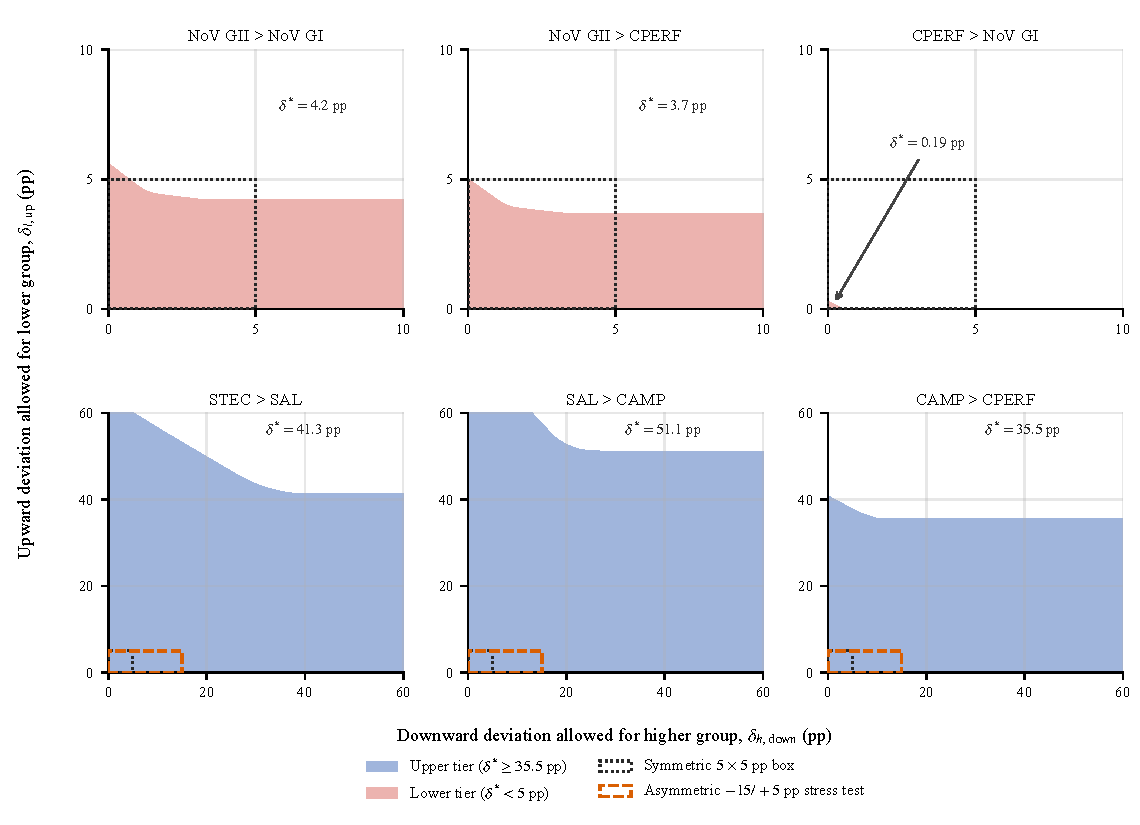
\includegraphics[width=0.95\linewidth]{figures/fig_04_calibrated_2d.pdf}
  \caption{Two-dimensional asymmetric sensitivity across all 15 pathogen pairs (higher group at $\delta = 0$ first). Shaded regions denote combinations of downward deviation allowed for the higher group ($\delta_{h,\text{down}}$) and upward deviation allowed for the lower group ($\delta_{l,\text{up}}$) preserving separation. Dotted and dashed boxes illustrate the symmetric $5 \times 5$ pp and asymmetric $-15/+5$ pp scenario stress tests.}
  \label{fig:cal2d}
\end{figure}

\subsection{30-Hypothesis Inference, State Clustering, Calibration and Rank Sets}\label{sec:res-inference}

High single-outbreak concentration explained skewed upper-bound sampling variance (Supplementary Table S7): maximum stratum case shares reached 69.2\% for \textit{C. perfringens} (max HHI $0.501$, $N_{\text{eff}} = 2.00$), 62.1\% for norovirus GI ($0.508$, $N_{\text{eff}} = 1.97$), 65.5\% for \textit{Campylobacter} ($0.491$, $N_{\text{eff}} = 2.04$) and 63.3\% for STEC ($0.479$, $N_{\text{eff}} = 2.09$) versus 33.0\% for \textit{Salmonella} ($0.133$, $N_{\text{eff}} = 7.49$). Across 33 states with $\ge 500$ common-support cases, unrecorded status spanned 0.0\%--40.3\% (median 12.2\%), and the top three states held 91.4\% of unrecorded STEC cases, 65.1\% for \textit{Salmonella} and 63.4\% for \textit{C. perfringens}; 53-state clustering scaled lower-difference SEs by factors of 0.77 to 1.73 (largest for STEC vs.\ \textit{Salmonella}, $1.73$).

Across all 30 ordered two-sided hypotheses (Table~\ref{tab:joint_inference}; Figure~\ref{fig:inference_followup}a), STEC above norovirus GII remained statistically significant without unrecorded-outcome assumptions under every inferential procedure: outbreak-HC1 Gaussian Max-$T$ ($c_{\text{sim},30} = 2.611$, $p_{\text{FWER}} = 0.0245$, IM 95\% CI $[+3.2, +39.2]$ pp), 2,000-replicate bootstrap covariance Gaussian Max-$T$ ($c = 2.617$, $p = 0.0315$), 53-state clustering ($c = 2.536$, $p = 0.0332$, state IM 95\% CI $[+2.9, +44.5]$ pp), 53-state wild cluster bootstrap ($p_{\text{WCB}} = 0.0306$), and studentized non-Gaussian bootstrap Max-$T$ ($c_{\text{boot}} = 2.725$, $p = 0.0430$). Under the $\delta = 5$ pp band ($c_{\text{sim},30} = 2.730$ HC1, $2.683$ state, $2.899$ non-Gaussian bootstrap), all 12 upper-tier orderings were jointly significant across Gaussian HC1 ($p < 0.001$), 53-state ($p < 0.001$), WCB ($p \le 0.0002$), and studentized non-Gaussian bootstrap Max-$T$ (maximum $p = 0.0020$ for \textit{Campylobacter} above norovirus GI; $p \le 0.0010$ for the other 11 pairs). Under the asymmetric $-15/+5$ pp band, all 12 upper-tier orderings likewise remained jointly significant under both HC1 and 53-state 30-hypothesis FWER ($p \le 0.0001$). Using dynamic $c_{\text{sim},30}(\delta)$, simultaneous 95\% confidence tipping points were $\infty$ for STEC above norovirus GII, 73.2--80.6 pp (HC1) / 77.3--90.3 pp (state) for STEC vs.\ \textit{Campylobacter}, \textit{C. perfringens} and norovirus GI, and 18.5--57.7 pp (HC1) / 18.0--54.7 pp (state) for the other upper-tier pairs ($\le 1.3$ pp for bottom three).

Simultaneous 95\% rank confidence sets across all five worst-case procedures yielded $[1, 5]$ for STEC, $[2, 6]$ for norovirus GII, and $[1, 6]$ for the remaining four groups. Under both $\delta = 5$ pp and the asymmetric $-15/+5$ pp scenario, the joint 95\% rank sets separated STEC $[1, 1]$, \textit{Salmonella} $[2, 2]$ and \textit{Campylobacter} $[3, 3]$ from the indistinguishable lower tier $[4, 6]$ across every inferential method.

In the 500-replicate bootstrap-world calibration preserving $n_{js}$ (Supplementary Table S8), asymptotic HC1 under-covered in sparse $N_{\text{eff}} \approx 2$ strata (IM 95\% empirical boundary coverage 76.4\% min, 87.4\% median; ratio of mean HC1 SE to MC SD 0.754--1.024). Empirical 30-hypothesis FWER rejection rates at nominal 5\% were: 32.8\% (HC0), 29.8\% (HC1), 25.6\% (non-Gaussian bootstrap critical value), 21.4\% (53-state clustering) and 20.6\% (wild cluster bootstrap) under worst-case bounds, falling to 20.8\%, 18.0\%, 12.6\%, 8.8\% and 8.0\% at $\delta = 5$ pp. Thus, accounting for state correlation and skewness improves calibration substantially, though anti-conservative finite-sample error persists in sparse highly concentrated strata.

\begin{table}[!tbp]
\centering
\scriptsize
\setlength{\tabcolsep}{2.3pt}
\renewcommand{\arraystretch}{1.12}
\caption{Joint M-estimation inference for the 15 pairwise standardized differences combining outbreak-HC1 and 53-state-clustered sandwich covariances, Imbens--Manski 95\% CIs, 200,000-draw Gaussian multiplier Max-T FWER p-values, and dynamic simultaneous 95\% confidence tipping points.}
\label{tab:joint_inference}
\begin{tabular}{>{\raggedright\arraybackslash}p{2.4cm}>{\raggedleft\arraybackslash}p{1.95cm}>{\raggedleft\arraybackslash}p{2.05cm}>{\raggedleft\arraybackslash}p{2.2cm}>{\raggedleft\arraybackslash}p{2.2cm}>{\raggedleft\arraybackslash}p{1.05cm}>{\raggedleft\arraybackslash}p{2.25cm}}
\toprule
Ordering at $\delta$ = 0 & ID bounds (pp) & IM 95\% CI (pp) & HC1 FWER p (w / $\delta$=5) & State FWER p (w / $\delta$=5) & $\delta^{*}$ (pt) & 95\% $\delta^{*}$ (HC1 / State) \\
\midrule
STEC $>$ CAMP & [+5.5, +29.3] & [+0.2, +33.3] & 0.260 / <0.001 & 0.115 / <0.001 & $\infty$ & 75.4 / 83.9 \\
STEC $>$ CPERF & [+5.0, +36.4] & [-2.5, +40.1] & 0.572 / <0.001 & 0.518 / <0.001 & $\infty$ & 76.6 / 78.2 \\
STEC $>$ NoV GI & [+6.0, +36.3] & [-1.0, +40.1] & 0.393 / <0.001 & 0.186 / <0.001 & $\infty$ & 82.2 / 91.2 \\
STEC $>$ NoV GII & [+7.5, +35.4] & [+3.2, +39.2] & 0.018 / <0.001 & 0.027 / <0.001 & $\infty$ & $\infty$ / $\infty$ \\
SAL $>$ NoV GII & [-2.7, +30.4] & [-6.3, +33.6] & 1.000 / <0.001 & 1.000 / <0.001 & 81.6 & 58.6 / 55.4 \\
SAL $>$ NoV GI & [-4.2, +31.3] & [-10.7, +34.5] & 1.000 / <0.001 & 1.000 / <0.001 & 76.5 & 48.3 / 50.4 \\
SAL $>$ CPERF & [-5.2, +31.3] & [-12.3, +34.6] & 1.000 / <0.001 & 1.000 / <0.001 & 72.1 & 45.0 / 43.6 \\
SAL $>$ CAMP & [-4.7, +24.2] & [-9.4, +27.8] & 1.000 / <0.001 & 1.000 / <0.001 & 51.1 & 21.5 / 19.3 \\
STEC $>$ SAL & [-7.0, +22.2] & [-11.1, +26.0] & 1.000 / <0.001 & 1.000 / <0.001 & 41.3 & 20.1 / 20.6 \\
CAMP $>$ NoV GI & [-11.2, +18.8] & [-17.9, +23.4] & 1.000 / <0.001 & 1.000 / <0.001 & 37.8 & 20.9 / 22.1 \\
CAMP $>$ NoV GII & [-9.7, +17.9] & [-13.4, +22.5] & 1.000 / <0.001 & 1.000 / <0.001 & 37.1 & 21.3 / 20.8 \\
CAMP $>$ CPERF & [-12.2, +18.9] & [-19.5, +23.4] & 1.000 / <0.001 & 1.000 / <0.001 & 35.5 & 19.2 / 18.6 \\
NoV GII $>$ NoV GI & [-17.4, +16.8] & [-23.9, +20.2] & 1.000 / 0.931 & 1.000 / 0.938 & 4.2 & 1.5 / 1.5 \\
NoV GII $>$ CPERF & [-18.4, +16.8] & [-25.5, +20.2] & 1.000 / 0.963 & 1.000 / 0.962 & 3.7 & 1.0 / 1.0 \\
CPERF $>$ NoV GI & [-18.3, +19.3] & [-24.8, +26.4] & 1.000 / 1.000 & 1.000 / 1.000 & 0.19 & 0.00 / 0.00 \\
\bottomrule
\end{tabular}
\par\smallskip\parbox{0.97\linewidth}{\footnotesize Outbreak-HC1 critical values: c\_sim = 2.49 (worst case), 2.53 ($\delta$ = 5); state-clustered: 2.46 / 2.49 (wild cluster bootstrap STEC $>$ NoV GII p = 0.028). 95\% $\delta^{*}$ uses dynamic c\_sim($\delta$). Simultaneous 95\% rank confidence sets at $\delta$ = 5: STEC [1,1]; SAL [2,2]; CAMP [3,3]; NoV GII [4,6]; CPERF [4,6]; NoV GI [4,6] (worst case: STEC [1,5], NoV GII [2,6], others [1,6]).}
\end{table}


\begin{figure}[!tbp]
  \centering
  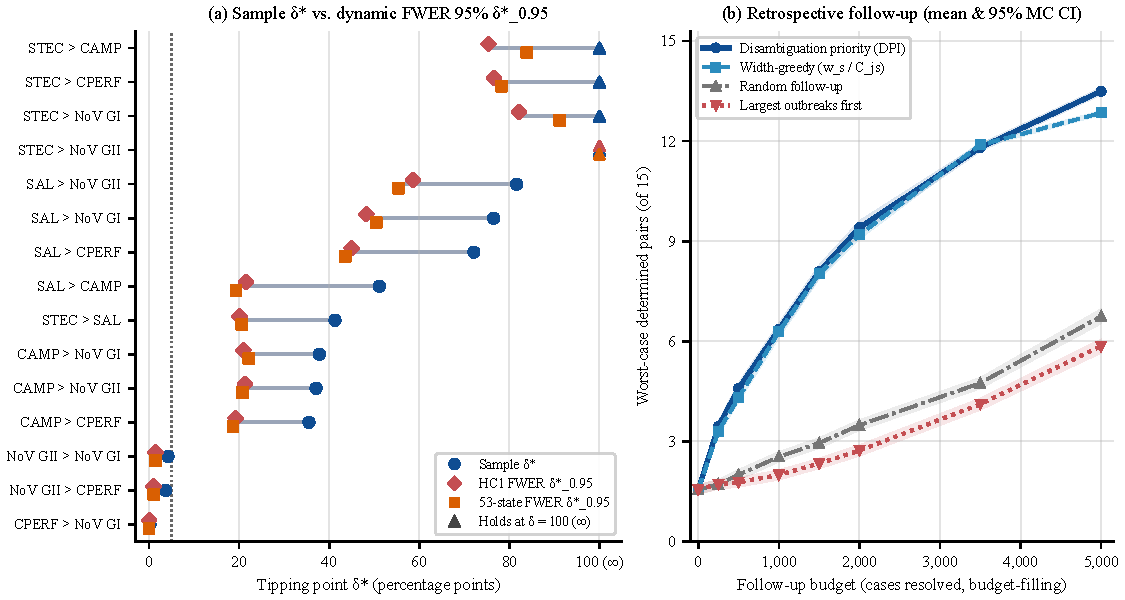
\includegraphics[width=0.96\linewidth]{figures/fig_05_inference_followup.pdf}
  \caption{Simultaneous 30-hypothesis confidence tipping points and cost-conditional follow-up benchmarks. (a) Sample tipping point $\delta^{*}$ versus dynamic 30-hypothesis FWER 95\% tipping points $\delta^{*}_{0.95}$ under outbreak-HC1 and 53-state clustering. (b) Per-case cost model (budget in cases resolved, budget-filling). (c) Per-outbreak cost model (budget in outbreaks contacted), illustrating strategy reversal between per-case and per-outbreak costs and unified optimality of Eq.~\ref{eq:followup}.}
  \label{fig:inference_followup}
\end{figure}

\subsection{Cost-Conditional Follow-Up Benchmarks and Sensitivity Variants}\label{sec:res-voi}

Evaluating Eq.~\ref{eq:followup} across 200 budget-filling masking trials on 2,414 fully recorded outbreaks (45,249 cases; baseline mean 1.55 determined pairs) revealed a sharp dependence on follow-up cost structure (Figure~\ref{fig:inference_followup}b--c; Supplementary Table S10). Under a per-case cost budget (1,000 cases), per-case stratum leverage $w_s/C_{js}$ resolved 6.29 pairs (95\% CI $[6.09, 6.48]$), more than doubling random follow-up (2.54 pairs, $[2.38, 2.69]$) and tripling largest-outbreak-first (2.00 pairs, $[1.84, 2.15]$; mean leverage $0.0088$ vs.\ $0.0573$ pp/case). Conversely, under a per-outbreak cost budget (100 outbreaks contacted), largest-outbreak-first reversed rank and strongly beat both random follow-up (7.90 vs.\ 3.27 pairs) and per-case $w_s/C_{js}$ (7.38 pairs), while the cost-optimal per-outbreak width rule $w_s U_i/C_{js}$ dominated all strategies (9.12 pairs, $[9.00, 9.23]$ at 100 outbreaks; 6.41 vs.\ 1.92--4.01 at 25 outbreaks). Under a mixed cost model ($\text{cost}_i = 20 + U_i$ case-equivalents; Supplementary Figure S3a), mixed cost-normalized targeting achieved the highest resolution at 1,000 units (4.09 pairs vs.\ 3.73 per-case, 3.57 per-outbreak, 1.95 largest-first, 1.94 random) and 2,000 units (6.24 vs.\ 4.74–5.05). Supplementary sensitivity checks confirm that heuristic DPI adds $+0.07$ pairs (95\% CI $[-0.07, +0.21]$) over $w_s/C_{js}$ in single-shot ranking, improves under 250-case adaptive tranches (7.31 at 1,000 cases), and preserves gains under MNAR, state-clustered, and 70\%-yield masking (Supplementary Figure S3b; real-data strata ranked in Supplementary Table S11; descriptive worst-case width decomposition in Supplementary Table S9).

Across all 17 cohort and specification sensitivity variants (Supplementary Table S5; Supplementary Figure S2), 4 to 7 pairs held without unrecorded-outcome assumptions and 12 to 14 at $\delta = 5$ pp, with zero reversals among the four primary pairs and only five variants (R1a, R2, R4a, R5, R6b) shifting a single low-tier $\delta = 0$ direction. Restricting exclusively to the 3,659 single-state outbreaks (variant R11) kept the identical 12 common-support cells, 4 worst-case pairs and 12 $\delta = 5$ pairs (zero changes vs.\ main). Including suspected etiologies (R8; 5,084 outbreaks, 16 cells) gave 5 / 13 pairs; excluding 79 healthcare outbreaks (R9) gave 4 / 12 (zero changes); and equal outbreak-level within-cell weighting (R10) gave 7 / 14 (zero reversals). Bootstrap resampling (Table~\ref{tab:pairwise}; Supplementary Table S6) determined the four primary worst-case orderings in 91.6\%--100.0\% of replicates ($0/2,000$ replicates lacked $K_{\text{rec}}$).
